\documentclass[11pt,a4paper,twocolumn]{article}

% ISB wants ARIAL but that is a MS font which can only be used with LauTeX or
% XeLaTeX, so helvetica is the next best thing. Damn this makes the paper
% longer than 2 pages!
\usepackage{helvet}
\renewcommand{\familydefault}{\sfdefault}

% TODO : The header still isn't quite right. I need to adjust the top
% margin only on the first page.
\usepackage[top=0.6in,bottom=0.5in,left=0.5in,right=0.5in,headsep=0pt,headheight=35pt]{geometry}

% for images: png, pdf, etc
\usepackage{graphicx}

% for nice table formatting, i.e. /toprule, /midrule, etc
\usepackage{booktabs}

% for nice units
\usepackage{siunitx}

% for more maths
\usepackage{amsmath}

% need to force 11 point font
\newcommand*{\ElevenPtFont}{%
      \fontsize{11}{20}%
      \selectfont}

% add in the conference header
\usepackage{fancyhdr}

\fancypagestyle{firststyle}
{
   \fancyhf{}
   \renewcommand{\headrulewidth}{0pt}
   \fancyhead[R]{\ElevenPtFont\textbf{XV International Symposium on Computer Simulation in Biomechanics}\\
     \textbf{July 9th--11th 2015, Edinburgh, UK}}
}

% the reference section header need to be all caps
\renewcommand{\refname}{\ElevenPtFont REFERENCES}

\title{\ElevenPtFont\textbf{QUIET STANDING CONTROL PARAMETER IDENTIFICATION WITH DIRECT
  COLLOCATION}}

\author{Jason K. Moore and Antonie van den Bogert\\
Mechanical Engineering, Cleveland State University, Cleveland, OH, USA\\
Email: moorepants@gmail.com, Web: http://hmc.csuohio.edu}

\date{}

\begin{document}

\maketitle

\thispagestyle{firststyle}

\section*{\ElevenPtFont INTRODUCTION}

It is hypothesized that a human operating during the quiet standing task uses
feedback to remain upright in the face of perturbations. For various reasons,
it is desirable to obtain mathematical models that predict a human's actuation
patterns given measured estimates of the sensory information available to the
human. Reasonably good models of the human's open loop musculoskeletal system
exist but models of the human's control system and the system process noises
are less than adequate. The control model can possibly be derived from first
principles, but high level understanding of the human's sensory neurological
feedback patterns are difficult to derive from the low level neurological first
principles. These high level control descriptions may be more easily arrived at
through optimal identification.

Here we present a numerical study demonstrating the merits of using a direct
collocation formulation to identify the parameters of non-linear closed loop
system. Parameter identification via direct collocation is exquisitely
described in a paper by Betts and Huffman~\cite{Betts2003} but these methods
have not, to the authors' knowledge, been used for control parameter
identification in biological systems. We aim to show that direct collocation is
better suited to control parameter identification because computation times are
extremely lower than competing optimization methods and it is much less
sensitive to initial guesses than shooting.

\section*{\ElevenPtFont METHODS}

We make use of a common model of closed loop quiet standing taken from
\cite{Park2004}. The plant is a two dimensional two body joint torque driven
inverted pendulum with inertial characteristics of a human,
Fig.~\ref{fig:free-body-diagram}. The human's foot is attached rigidly to a
moving base which can be accelerated, thus the ankle joint has a prescribed
lateral motion. The open loop equations of motion of the system take this form
%
\begin{equation}
  0 = \mathbf{M}(\mathbf{x}, t) \dot{\mathbf{x}} - \mathbf{F}(\mathbf{x},
    \mathbf{u}, a, \mathbf{p}, t)
\end{equation}
%
where $\mathbf{M}$ is the mass matrix, $\mathbf{x}$ is the state, $\mathbf{F}$
is the forcing vector, $\mathbf{u}$ are the joint torques, $a$ is the platform
acceleration, $\mathbf{p}$ are the constant body segment parameters, and $t$ is
time.
%
\begin{figure}
  \centering
  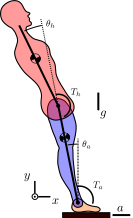
\includegraphics{figures/free-body-diagram.pdf}
  \caption{Free body diagram of plant model used in this study.}
  \label{fig:free-body-diagram}
\end{figure}

We then assume a controller that implements full state feedback based on a
reference of zero, i.e. upright standing. We model the human's inability to
perfectly sense this error by injecting Gaussian noise onto error. The
controller takes the form
%
\begin{equation}
  \mathbf{u} = \mathbf{K} (\mathbf{x}_n - \mathbf{x})
\end{equation}
%
where $\mathbf{K}$ is the time invariant gain matrix and $\mathbf{x}_n$ is the
reference noise.

We simulate the closed loop model with optimal gains take from \cite{Park2004}
to generate measurement data. The simulation requires the exogenous input, $a$,
to be specified for the time duration. We specify $a$ to be a sum of sines to
perturb the system. The measured data of interest includes the system state and
the platform acceleration, all of which have measurement noise $\mathbf{v}$
applied before identification.
%
\begin{align}
  \mathbf{x}_m = [\mathbf{\theta}, \mathbf{\omega}]^T + [\mathbf{v}_\theta,
  \mathbf{v}_\omega]^T \\
  a_m = a + v_a
\end{align}

We then construct an identical model, except without the process noise, for
parameter identification purposes. We formulate the optimal control problem by
direct collocation to minimize this model's trajectory with respect to the
``measured'' data from above. The cost function is simply
%
\begin{equation}
  J(\mathbf{x}, \mathbf{K}) = \int_{t_0}^{t_f}[\mathbf{x}_m(t) - \mathbf{x}(t)]^2 dt
\end{equation}
%
and subject to the constraints
%
\begin{equation}
  \mathbf{c}(\mathbf{x}, \mathbf{K}) = \mathbf{M} \dot{\mathbf{x}} -
  \tilde{\mathbf{F}}(\mathbf{x},
  a_m, \mathbf{p}, \mathbf{K}, t)
\end{equation}
%
where $\tilde{\mathbf{F}}$ is the closed loop forcing vector.

We make use of first order midpoint integration to discretize the system at $N$
nodes from $t_0$ to $t_f$. This constrained optimization problem has $4N + 8$
unknowns and is subject to $4(N-1)$ constraint equations. Our initial guess for
the state trajectories and the controller gains is zero and we use a large
scale interior point optimization routine to minimize the cost function.

All of the above is implemented with several open source software packages tied
together with the Python programming language. The equations of motion are
derived with SymPy and the model is simulated at 10x real time speeds with PyDy
to generate the measurement data. The constraint equations and their sparse
Jacobians are formulated symbolically with opty and efficient wrapped C code is
generated to evaluate them numerically. Finally, IPOPT is used to solve the
optimization problem.

\section*{\ElevenPtFont RESULTS}

For an example result we simulate the closed loop model for a duration of 20
seconds under the influence of a platform acceleration with a standard
deviation of 3.6~\si{\meter\per\second\squared} and assume that the reference
noise, $\mathbf{x}_n$ is zero. Gaussian measurement noise is then added
to the state trajectories ($\sigma_\theta=0.005$ \si{\radian} and
$\sigma_\omega=0.07$ \si{\radian\per\second}) and acceleration $\sigma_a=0.4$
\si{\meter\per\second\squared} to produce the simulated measurements used for
identification. We then set up a direct collocation problem discretized with
$N=6001$ nodes, creating a problem with $24012$ free variables. Given an
initial guess of all zeros for the states and the unknown parameters, the
solution is found after 27 iterations which only takes approximately seven
seconds on a four core Intel Core i5 processor.

Figure~\ref{fig:trajectory-comparison} shows a comparison of the measured state
trajectories and the optimal trajectories and Table~\ref{tab:relative-error}
provides the percent relative error in the identified gains with respect to the
known gains.
%
\begin{figure}
  \centering
  \includegraphics[width=\columnwidth]{figures/trajectory-comparison.pdf}
  \caption{A comparison of the measured states, black dots, and the identified
    states, solid lines.}
  \label{fig:trajectory-comparison}
\end{figure}
%
\begin{table}
  \centering
  \caption{The percent relative error of the identified gains with respect to
    the known gains.}
  \begin{tabular}{lrrrr}
  \toprule
        & $\theta_a$ & $\theta_h$ & $\omega_a$ & $\omega_h$ \\
  \midrule
  $T_a$ & 1.822 & -3.412 & -1.097 & -0.887 \\
  $T_h$ & 6.346 & -0.617 & -0.251 & 0.346  \\
  \bottomrule
\end{tabular}
  \label{tab:relative-error}
\end{table}

\section*{\ElevenPtFont DISCUSSION}

The indirect control parameter identification via direct collocation has
several advantages to more common nonlinear parameter identification methods.
Firstly, it handles unstable systems with ease whereas single and multiple
shooting often fail miserably with an unstable simulation. This makes the
algorithm much less sensitive to poor initial guesses. Some evolutionary
algorithms are able to home in on the optimal solution from a random initial
guess but take many iterations and hours of parallel computation time.  And
lastly, computation speeds are a tiny fraction of various shooting algorithms.
This method does not require the equations of motion to be in explicit first
order form which saves computation time. Our formulation correctly identifies
the parameters in approximately the time a single shooting iteration may take.
The main limitations here are the requirement that the constraints are
continuously differentiable and there could be memory issues if the number of
nodes is extremely high, i.e. a long measurement duration.

%The demonstration at the conference will include comparisons to other popular
%optimization algorithms, more details of how to deal with process noise, and
%several other parameter and trajectory optimization problems that can be
%handled by the open source software suite we have developed.

\bibliographystyle{unsrt}
\bibliography{references}

\end{document}
